%**************************************************************************
%*
%*  Instrucciones para la platilla del informe final
%*
%*  
%*
%*  Filename: platillapaper.tex
%*
%*
%*  
%*  
%*
%**************************************************************************


\documentclass{wscpaperproc}
\usepackage[spanish]{babel}
\usepackage{latexsym}
\usepackage{graphicx}
\usepackage{mathptmx}
\usepackage[T1]{fontenc}
\usepackage{listings}

%****************************************************************************
% AUTHOR: You may want to use some of these packages. (Optional)
\usepackage{amsmath}
\usepackage{amsfonts}
\usepackage{amssymb}
\usepackage{amsbsy}
\usepackage{amsthm}
%****************************************************************************


%
%****************************************************************************
% AUTHOR: If you do not wish to use hyperlinks, then just comment
% out the hyperref usepackage commands below.

%% This version of the command is used if you use pdflatex. In this case you
%% cannot use ps or eps files for graphics, but pdf, jpeg, png etc are fine.

\usepackage[colorlinks=true,urlcolor=blue,citecolor=black,anchorcolor=black,linkcolor=red]{hyperref}
%\usepackage{hyperref}

%% The next versions of the hyperref command are used if you adopt the
%% outdated latex-dvips-ps2pdf route in generating your pdf file. In
%% this case you can use ps or eps files for graphics, but not pdf, jpeg, png etc.
%% However, the final pdf file should embed all fonts required which means that you have to use file
%% formats which can embed fonts. Please note that the final PDF file will not be generated on your computer!
%% If you are using WinEdt or PCTeX, then use the following. If you are using
%% Y&Y TeX then replace "dvips" with "dvipsone"

%%\usepackage[dvips,colorlinks=true,urlcolor=blue,citecolor=black,%
%% anchorcolor=black,linkcolor=black]{hyperref}
%****************************************************************************


%
%****************************************************************************
%*
%* AUTHOR: YOUR CALL!  Document-specific macros can come here.
%*
%****************************************************************************

% If you use theoremes
\newtheoremstyle{wsc}% hnamei
{3pt}% hSpace abovei
{3pt}% hSpace belowi
{}% hBody fonti
{}% hIndent amounti1
{\bf}% hTheorem head fontbf
{}% hPunctuation after theorem headi
{.5em}% hSpace after theorem headi2
{}% hTheorem head spec (can be left empty, meaning `normal')i

\theoremstyle{wsc}
\newtheorem{theorem}{Teorema}
\renewcommand{\thetheorem}{\arabic{theorem}}
\newtheorem{corollary}[theorem]{Corolario}
\renewcommand{\thecorollary}{\arabic{corollary}}
\newtheorem{definition}{Definici\'on}
\renewcommand{\thedefinition}{\arabic{definition}}


%#########################################################
%*
%*  The Document.
%*
\begin{document}

%***************************************************************************
% AUTHOR: AUTHOR NAMES GO HERE
% FORMAT AUTHORS NAMES Like: Author1, Author2 and Author3 (last names)
%
%		You need to change the author listing below!
%               Please list ALL authors using last name only, separate by a comma except
%               for the last author, separate with "and"
%
\WSCpagesetup{Acosta, Valles, Pirchardo, de la Torre, and Barcenas }

% AUTHOR: Enter the title, all letters in upper case
\title{T\'itulo}

% AUTHOR: Enter the authors of the article, see end of the example document for further examples
\author{Rafael Acosta M\'arquez\\[12pt]
	Grupo C211\\
	Ciencia de la Computaci\'on\\
	Facultad de Matem\'atica y Computaci\'on\\
	Universidad de La Habana. Cuba\\
% Multiple authors are entered as follows.
% You may also need to adjust the titlevbox size in the preamble - search for titlevboxsize
\and
Eisler F. Valles Rodr\'iguez\\[12pt]
Grupo C211\\
	Ciencia de la Computaci\'on\\
	Facultad de Matem\'atica y Computaci\'on\\
	Universidad de La Habana. Cuba\\
\and
Jorge Pichardo Cabrera\\[12pt]
Grupo C212\\
    Ciencia de la Computaci\'on\\
	Facultad de Matem\'atica y Computaci\'on\\
	Universidad de La Habana. Cuba\\
\and
Orlando Rafael de la Torre Leal\\[12pt]
Grupo C211\\
	Ciencia de la Computaci\'on\\
	Facultad de Matem\'atica y Computaci\'on\\
	Universidad de La Habana. Cuba\\
\and
Ernesto Alejandro B\'arcenas Trujillo\\[12pt]
Grupo C211\\
    Ciencia de la Computaci\'on\\
	Facultad de Matem\'atica y Computaci\'on\\
	Universidad de La Habana. Cuba\\
}


  

\maketitle
\newpage

\section*{Resumen}
Aqu\'i va el resumen del trabajo en esta plantilla  \LaTeX\ 

\section{INTRODUCCI\'ON}
El presente art\'iculo, escrito por Roberto Pradas Velasco, Fernando Antoñanzas Villar, Javier Mar, fue publicado en a revista Gaceta Sanitaria en el año 2009. 
Dicha revista  contaba con un factor de impacto de 1.172 en el a\~no 2009 y tuvo un factor de impacto de 2.479 en el a\~no 2022, lo que indica su 
relevancia en el \'ambito acad\'emico.
El art\'iculo trata sobre la utilizaci\'on conjunta de \'arboles de decisi\'on y modelos epidemiol\'ogicos basados en ecuaciones
diferenciales como un m\'etodo apropiado para la evaluaci\'on econ\'omica de medidas profil\'acticas ante
enfermedades infecciosas. Estos modelos permiten combinar el comportamiento din\'amico de la
enfermedad con el consumo de recursos sanitarios. Para ilustrar este tipo de modelos se ajusta un sistema
din\'amico de ecuaciones diferenciales al comportamiento epid\'emico de la gripe en España, con el fin de
proyectar el impacto epidemiol\'ogico de la vacunaci\'on antigripal. Nosotros recreamos los experimentos realizados para hallar las soluciones 
al sistema en los distintos instantes de tiempo $t \in [1,52] $
\label{sec:intro}

\section{Resultados fundamentales}
\subsection{Estructura del trabajo}
Dado que el objetivo de el paper analizdo es presentar de forma guiada la
construcción de un modelo dinámico, cuyo funcionamiento y resultados se ilustrarán mediante una aplicación a la evaluación
económica de la vacunación antigripal en España, en este art\'iculo simularemos los pasos
mostrados para analizar el comportamiento de una hip\'otetica epidemia gripal,
para ello dividiremos la poblacio\'on en las siguientes categor\'ias:
susceptibles(Aquellos individuos que están en condiciones de ser contagiados),
infectivos (aquellos que infectan o pueden
infectar a los susceptibles) y por último los resistentes (los que presentan
resistencia al agente infeccioso al recuperarse de la enfermedad ya sea por inmunización natural
o al quedar inmunizados por la vacuna).
\\
Basados en esto se plantea el siguiente sistema no lineal de ecuaciones diferenciales ordinarias

\begin{equation}
\hspace{-7em}
\begin{aligned}
\left\{
\begin{array}{l}
S'(t) = -\beta*I(t)*S(t)-V(t) \\
R'(t) = -\beta*I(t)*S(t)- \gamma*I(t); \ siendo \ N = S(t)+I(t)+R(t)\\
I'(t) = \gamma*I(t)+ V(t)
\end{array}
\right.
\end{aligned}
\end{equation}

Donde N es el tamaño de la población considerada, en este caso N =100'000,
S(t),I(t) y R(t) representan el número de susceptibles, infectivos y resistentes en cada instante de tiempo t.
$\beta$ es el coeficiente de transmisión  y $\gamma$ el coeficiente de retiro natural el cual 
es un indicador del ritmo con el cual los contagiados dejan de ser infectivos, además de esto
se tienen las derivadas de primer orden respecto a t S'(t), R'(t) e I'(t)
Para resolver este sistema es necesario los valores iniciales de cada una de 
las categorias en las cuales se dividió la población inicialmente además de los valores de los coeficientes
de retiro y de transmisión, en este caso se toman valores que concuerden con datos ya observados
como lo son el coeficiente de retiro natural $\gamma = 3.47$ y el coeficiente de transmisión
$\beta = \frac{\gamma}{96'015} = \frac{3,47}{96'015}$ donde 96'015 es el número
de susceptibles en el auge de la onda epidémica, que se ha obtenido reduciendo proporcionalmente
la cifra en la población española para ajustar el comportamiento
del modelo a un colectivo de 100'000 individuos. Se ha escogido
este tamaño poblacional (N) por ser un valor empleado con
frecuencia en las fuentes de información epidemiológica, y
además porque facilita la interpretación y el cálculo de los
indicadores económicos del estudio.\\
Según la distribución por clases de la población en la primera
semana del período epidemiólgico estudiado (semana 0), los
valores iniciales para la resolución del sistema de ecuaciones
diferenciales son los siguientes:

\begin{equation}
\hspace{-14cm}
\begin{aligned}
\left\{
\begin{array}{l}
S(0) = 99986 \\
R(0) = 14 \\
I(0) = 0
\end{array}
\right.
\end{aligned}
\end{equation}
El número de infectivos en la primera semana, I(0) = 14, es un
valor promedio basado en series históricas de la enfermedad,
cedidas por el Centro Nacional de Epidemiología.\\
La forma de la función de vacunación V(t) se ha definido 
considerando el impacto de la vacunación en la reducción del
número de susceptibles. Se ha tenido en cuenta el número de
individuos que han sido vacunados de manera efectiva, es decir,
aquellos que han experimentado los efectos positivos de la vacuna
según su eficacia. La vacunación se ha incorporado gradualmente utilizando
 una función definida por intervalos con el siguiente formato:

\begin{equation}
\hspace{-28em}
V(t)=
\begin{aligned}
\left\{
\begin{array}{l}
	0 \ si\  0 \le t \le 9 \\
	V \ si\  9 < t \le 18 \\
	0 \ si\  18 < t \le 51 \\
\end{array}
\right.
\end{aligned}
\end{equation}

Donde V  representa el número de vacunados semanalmente, aquí tomamos
el tiempo medido en semanas y el período epidemiológico de estudio es el
año epidemiológico de la gripe(52 semanas).
Recalcar aquí que en el intervalo donde V(t) no es nula no coincide
 con el asociado a la campaña de vacunación (octubre y
noviembre), sino que está diferido 2 semanas, que es el tiempo
medio que tarda la vacuna en producir la inmunidad del individuo
vacunado. La cantidad de individuos vacunados cada semana se calcula como:\\

$V = \frac{Nv\epsilon}{9}$

donde v  y $\epsilon$ son el índice per cápita de vacunación(cobertura vacunal) e índice
per cápita de la eficacia de la vacuna respectivamente.
Realmente la vacunación actúa haciendo que parte de
los individuos que eran susceptibles pasen a ser resistentes, y con
ello se reduce la posibilidad de contagio al decaer el número de
contactos entre susceptibles e infectivos, esto se refleja en la figura 4



\subsection[short]{M\'etodos y algoritmos utilizados}

Para corroborar los resultados mostrados en este paper,
se us\'o el m\'etodo de Runge-Kutta de 4to orden (RK4)
teniendo en cuenta la siguiente tabla de par\'ametros iniciales:


\begin{table}[htbp]
  \centering
  \caption{Valores iniciales usados en la simulación}
  \label{tabla-ejemplo}
  \begin{tabular}{|c|c|c|}
    \hline
    \textbf{Párametro} & \textbf{Valor} \\
    \hline
    Índice per cápita de cobertura vacunal, v & 0,20 \\
    Número total de individuos, N & 100'000\\
	Coeficiente de transmisión, $\beta$ & $ 3.614\times10^-5$\\
	Coeficiente de retiro natural, $\gamma$ & 3.47\\
	Índice per capita de eficacia de la vacuna, $\epsilon$ & 0.67\\
	Susceptibles iniciales &99'986\\
	Infectivos iniciales & 14\\
	Resistentes iniciales & 0\\
    \hline
  \end{tabular}
\end{table}

Estos resultados se muestran en la figura 1 y figura 2 donde se simula
el comportamiento tanto si se realiza la vacunación como si no, llegando
a los mismos resultados vistos en el paper analizado

\begin{figure}
	\centering
	\includegraphics[width=1.0\textwidth,height=5cm]{Figure_1.png}
	\caption{Gráficas en función del tiempo si se realiza la vacunación}

	\centering
	\includegraphics[width=1.0\textwidth,height=5cm]{Figure_2.png}
	\caption{Gráficas en función del tiempo si no se realiza la vacunación}\centering
  \end{figure}

\newpage

\begin{figure}
	\includegraphics[width=1.0\textwidth]{fig3.jpg}
	\caption{Diagrama de Fases }
\end{figure}

\begin{figure}
	\centering
	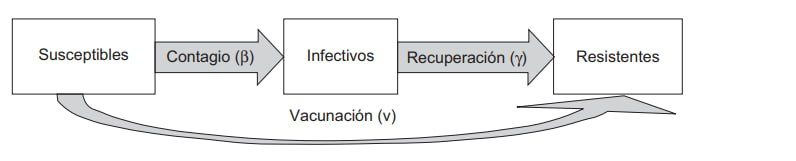
\includegraphics[width=1.0\textwidth,height=5cm]{fig4.jpg}
	\caption{Dinámica epidémica de la enfermedad.}
\end{figure}




\clearpage
\section*{Agradecimientos}


\appendix

\clearpage
\section{Anexos} \label{app:quadratic}
\begin{lstlisting}[language=python]
	def tamanno_poblacion <- 100000;
	def susceptibles <- 99986;
	def infectivos <- 14;
	def resistentes <- 0;
	def susceptibles_auge_onda_epidemica <- 96015;
	def coeficiente_retiro_natural <- 3.47;
	def eficacia_vacuna: float <- 0.67;
	def cobertura_vacunal: float <- 0.20;
	def coeficiente_transmision <- coeficiente_retiro_natural
		                     /susceptibles_auge_onda_epidemica;
	
	funcion edo(t, valores):
	 	(dx, dy, dz) <- valores;
		dxdt <- -coeficiente_transmision*dy*dx-Vacunados(t);
		dydt <- coeficiente_transmision*dy*dx
			   -coeficiente_retiro_natural*dy;
		dzdt <- coeficiente_retiro_natural*dy+Vacunados(t);
		retorna Arreglo(dxdt, dydt, dzdt);
	
	funcion Vacunados(tiempo):
		Si tiempo >= 0 y tiempo <= 9 Entonces
			retorna 0
		Si tiempo > 9 y tiempo <= 18 Entonces
			retorna tamanno_poblacion*eficacia_vacuna*
					cobertura_vacunal/9.0
		Si tiempo>18 Entonces
			retorna 0
	
	funcion runge_kutta4(f, x0, y0, h, n):
		ArregloSoluciones <- [(x0, y0)]
		Desde i=1 hasta n Hacer
			(xi, yi) <- ArregloSoluciones.UltimoElemento
			k1 <- h * f(xi, yi)
			k2 <- h * f(xi + h/2, yi + k1/2)
			k3 <- h * f(xi + h/2, yi + k2/2)
			k4 <- h * f(xi + h, yi + k3)
			y_next <- yi + (k1 + 2*k2 + 2*k3 + k4)/6
			x_next <- xi + h
			ArregloSoluciones.Annadir((x_next, y_next))
		Siguiente	

		retorna ArregloSoluciones

	Resultados = runge_kutta4(edo, 0, [99986, 14, 0], 1, 52)

\end{lstlisting}


\end{document}

